%Monolingual alignment models have been shown to boost the performance of question answering systems by "bridging the lexical chasm" between questions and answers.


\section{Alignment for question answering}
\label{sec-naacl2015:intro}
%\section{NAACL 2015 Related Work}
%\label{sec:related_work_naacl2015}
%\vspace{-2mm}


For the task of question answering (QA), lexical semantic models have shown promise in bridging \citet{Berger:00}'s "lexical chasm," or the lack of lexical overlap between questions and their answers.  In general, these models can be classified into alignment models \citep{echihabi2003noisy,Soricut:06,Riezler:etal:2007,Surdeanu:11,yao2013}, which are based on the repurposing of machine translation models to operate over aligned question-answer pairs within a single language (and hence require structured training data), and language models ~\citep{jansen14,sultan-etal:2014:TACL,yih13}, which operate over free text.  
This training data requirement of alignment models is their main limitation, as it is difficult to obtain in specialized domains or low-resource languages.
In this Chapter, we focus on closing this gap in resource availability by proposing two inexpensive methods for training alignment models solely using free text by generating artificial question-answer pairs from discourse structures. 
%Our approach is driven by two representations of discourse: a shallow sequential representation, and a deep one based on Rhetorical Structure Theory. 
%Here, we focus on closing this gap in resource availability by developing a method to train an alignment model over free text by making use of discourse structures. 

\subsection{Related Work}
Discourse has been previously applied to QA to help identify answer candidates that contain explanatory text (e.g. \citet{Verberne:2007} \todo{check ref} conducted an initial analysis of using discourse features derived from Rhetorical Structure Theory (RST)~\citep{mann88} for answer candidate selection, and concluded that while discourse features appeared useful, automated discourse parsing tools were required to test the idea on a larger scale.  
\citet{jansen14} proposed a reranking model that used both shallow and deep discourse features to identify answer structures in large answer collections across different tasks and genres.  Here we use discourse to impose structure on free text to create inexpensive knowledge resources for monolingual alignment. Our work is conceptually complementary to that of Jansen et al. -- where they explored largely unlexicalized discourse structures to identify explanatory text, we use discourse to learn lexicalized models for semantic similarity.

%\subsection{Artificial alignments}
Our work is conceptually closest to that of \citet{hickl2006recognizing}, who created artificially aligned pairs for textual entailment.  Taking advantage of the structure of news articles, wherein the first sentence tends to provide a broad summary of the article's contents, Hickl et al. aligned the first sentence of each article with its headline.  By making use of automated discourse parsing, here we go further and impose alignment structure over an entire text.

\subsection{Chapter overview}

The remainder of this Chapter is organized as follows.  In Section \ref{sec-naacl2015:approach} we describe our two approaches to generating artificially aligned text pairs.  Then, in Section \ref{sec-naacl2015:models} we describe our models and model features in more detail.  In Section \ref{sec-naacl2015:experiments} we detail the experimental setup used to evaluate the proposed models on two corpora from different genres and domains: one from Yahoo! Answers and one from the biology domain, and two types of non-factoid questions: manner and reason. In Section \ref{sec-naacl2015:results} we provide the results, showing that these alignment models trained directly from discourse structures imposed on free text
improve performance considerably over an information retrieval baseline and a neural network language model trained on the same data.  Finally, in Section \ref{sec-naacl2015:conclusion} we draw conclusions about our approach.

%
% Example of alignment models
%
%\begin{table}[t!]
%\begin{center}
%\begin{scriptsize}
%\begin{tabular}{l|p{60mm}}
%Passage	& Bob likes apples, which grow in his orchard.  He uses them for cider.  \\
%\hline
%Sequential & Bob likes apples, which grow in his orchard. $\rightarrow$ He uses them for cider. \\
%\hline
%RST & Bob likes apples, $\rightarrow$ which grow in his orchard. \\
% & Bob likes apples, which grow in his orchard. $\rightarrow$ He uses them for cider. \\
%
%
%\end{tabular}
%\end{scriptsize}
%%\vspace{-4mm}
%\caption{{\footnotesize \label{font-table} 
%An example of the alignments produced by the two discourse models.  While the sequential model aligns at sentence granularity capturing only intersentence information, the RST model aligns on finer EDU boundaries, capturing both inter/intrasentence alignments.
%}}
%\vspace{-4mm}
%
%\label{tab:examples}
%\end{center}
%\end{table}


\begin{figure}[t!]
\begin{center}
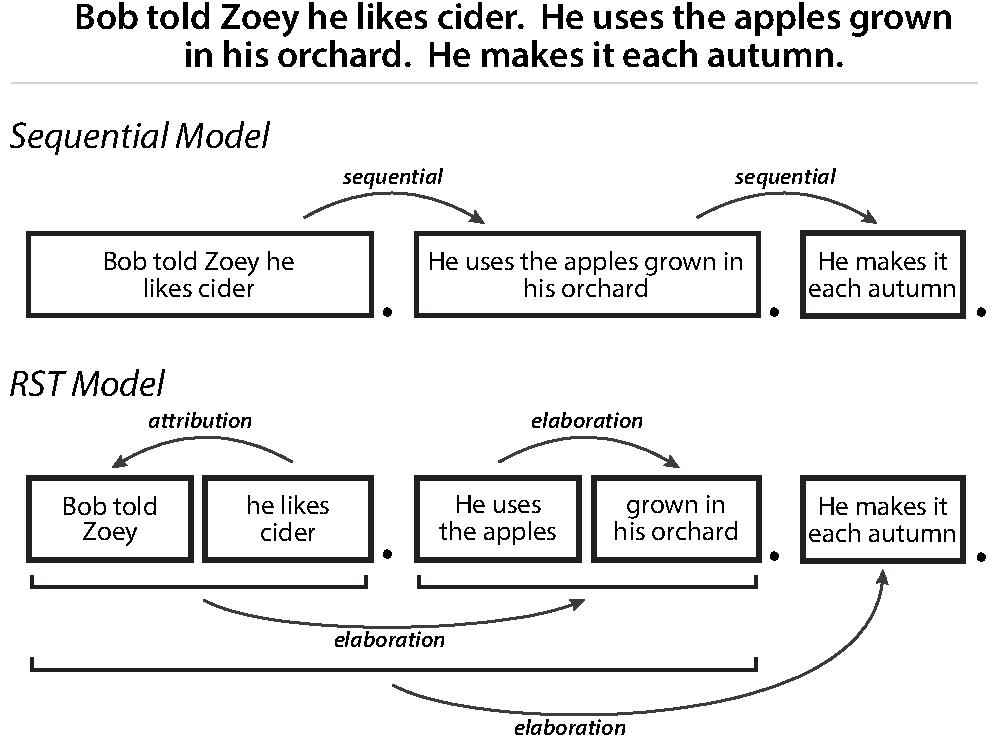
\includegraphics[width=100mm]{mainmatter/naacl2015-alignment/rst2a.pdf}
%space{-2mm}
\caption{{\small An example of the alignments produced by the two discourse models.  The sequential model aligns pairs of consecutive sentences, capturing intersentence associations such as \emph{cider--apples}, and \emph{orchard--autumn}.  The Rhetorical Structure Theory based model generates alignment pairs from participants in all (binary) discourse relations, capturing both intrasentence and intersentence alignments, including 
\emph{apples--orchard, cider--apples}, and \emph{cider--autumn}.}}
\label{fig:examples}
\end{center}
\end{figure}

\section{Approach}
\label{sec-naacl2015:approach}

A written text is not simply a collection of sentences, but rather a flowing narrative where sentences and sentence elements depend on each other for meaning -- a concept known as cohesion~\citep{halliday2014cohesion}.  
Here we examine two methods for generating alignment training data from free text that make use of cohesion: a shallow method that uses only intersentence structures, and a deep method that uses both intrasentence and intersentence structures.
We additionally attempt to separate the contribution of discourse from that of alignment in general by comparing these models against a baseline alignment model which aligns sentences at random.

The first model, the sequential discourse model (SEQ), considers that each sentence continues the narrative  of the previous one, and creates artificial question-answer pairs from all pairs of consecutive sentences.
% ms: no space
%This is similar to a right-attachment baseline in dependency parsing, 
%but operating at sentence granularity rather than word.
Thus, this model takes advantage of intersentence cohesion by aligning the content words\footnote{In pilot experiments, we found that aligning only nouns, verbs, adjectives, and adverbs yielded higher performance.} in each sentence with the content words in the following sentence.  For example, in the passage in Figure \ref{fig:examples}, this model would associate \emph{cider} in the first sentence with \emph{apples} and \emph{orchard} in the second sentence.

The second model uses Rhetorical Structure Theory (RST) to capture discourse cohesion both within and across sentence boundaries.  
We extracted RST discourse structures using an in-house parser~\citep{Surdeanu:15}, which follows the architecture introduced by \citet{hernault10} and \citet{feng12}.
The parser first segments text into elementary discourse units, which may be at sub-sentence granularity, then recursively connects neighboring units with binary discourse relations, such as \emph{Elaboration} or \emph{Contrast}.
%\footnote{The RST parser performs better on relations which occur more frequently.  We use only relations that occurred at least 1\% of the time.  This amounted to six relations: \emph{elaboration}, \emph{attribution}, \emph{background}, \emph{contrast}, \emph{same-unit}, and \emph{joint}. Using all relations slightly improves performance by 0.3\% P@1.} 
Our parser differs from previous work with respect to feature generation in that we implement all features that rely on syntax using solely dependency syntax. For example, a crucial feature used by the parser is the dominance relations of \citet{soricut2003}, which capture syntactic dominance between discourse units located in the same sentence. While originally these dominance relations were implemented using constituent syntax, we provide an equivalent implementation that relies on dependency syntax. The main advantage to this approach is speed: the resulting parser performs at least an order of magnitude faster than the parser of \citet{feng12}. 

Importantly, we generate artificial alignment pairs from this imposed structure by aligning the governing text (nucleus) with its dependent text (satellite).\footnote{Pilot experiments showed that this direction of alignment performed better than aligning from satellite to nucleus.} 
 Turning again to the example in Figure \ref{fig:examples}, this RST-based model captures additional alignments that are both intrasentence, e.g., \emph{apples--orchard}, and intersentence, e.g., {\em cider--autumn}. 
% intersentence associations of the sequential baseline, in addition it finds an intrasentence association between \emph{apples} and \emph{orchard}. 

%\todo{The random alignment baseline (RND) was created in a similar fashion to the SEQ model, except that the sentences were randomly shuffled first.  In the open domain this shuffling took place within a document, and in the biology domain it was done across the entire of the textbook.}
